\documentclass[pageno]{jpaper}

%replace XXX with the submission number you are given from the ASPLOS submission site.
% \newcommand{\asplossubmissionnumber}{171}

\usepackage[normalem]{ulem}

\input{libpaper/texheader}

\microtypecontext{spacing=nonfrench}

\usepackage{listings,multicol}
\usepackage{listings-rust}
\usepackage[scaled=0.85]{beramono}
\usepackage[T1]{fontenc}
\usepackage{hyperref}
\usepackage{xcolor}
\usepackage{amsthm}
\usepackage{amsmath}
\usepackage{amssymb}
\usepackage{dblfloatfix}

\theoremstyle{invar}
\theoremstyle{goal}
\newtheorem{invar}{Invariant}
\newtheorem{goal}{Design Goal}

%\usepackage{listings-rust}

\lstset{
    language=Rust, 
    style=boxed,
    basicstyle=\ttfamily,
    columns=fullflexible,
    breaklines=false,
    escapechar=\#,
    postbreak=\mbox{\textcolor{blue}{$\hookrightarrow$}\space},
}
% \lstset{language=Rust, style=colouredRust}
\newcommand{\hllr}[1]{\makebox[0pt][l]{\color{red!15}\rule[-3pt]{#1}{10pt}}}
\newcommand{\hll}[1]{\makebox[0pt][l]{\color{green!15}\rule[-3pt]{#1}{10pt}}}
\newcommand{\hlw}[1]{\makebox[0pt][l]{\color{green!35}\rule[-3pt]{#1}{10pt}}}

%auto-ignore

\newcommand{\papertitle}{\This{}: Statically-Enforced Persistent Memory Safety}

\newcommand{\this}{Corundum}
\newcommand{\This}{Corundum}
\newcommand{\lst}{\mathcal{L}}


%\lstMakeShortInline!

\lstnewenvironment{rust}{}{}


\newfloat{lstfloat}{t}{lop}
\floatname{lstfloat}{Listing}

%tighten bold paragraph
\renewcommand{\boldparagraph}[1]{\vspace*{0.5ex}\noindent\textbf{#1}\hspace{1em}}


\newenvironment{goaltrue}[1]{\begin{discuss}[Design Goal~\ref{#1} (\nameref{#1}) Holds:]}{\end{discuss}}% ignore macros

\newenvironment{discuss}[1][Details:]{\boldparagraph{#1}}{\vspace{1ex}}%$\blacksquare$}

\newcommand{\rerr}{{\color{red}\textbf{{\fontencoding{U}\fontfamily{futs}\selectfont\char 66\relax}}}}

\newcommand{\refl}[1]{Line~\ref{#1}}% ignore macros ignore misc
\newcommand{\reflr}[2]{Lines~\ref{#1}--\ref{#2}}% ignore macros ignore misc


\usepackage{adjustbox}
\usepackage{array}

\newcolumntype{R}[2]{%
    >{\adjustbox{angle=#1,valign=m,height=#2,padding*=0em -1.1em 0 0.2em}\bgroup}%
    l%
    <{\egroup}%
}
\newcolumntype{K}[2]{%
    >{\adjustbox{angle=#1,valign=m,height=(#2),padding*=0em -1.1em 0 0.2em}\bgroup}%
    l%
    <{\egroup}%
}
\newcommand*\rot{\multicolumn{1}{R{40}{2em}}}% no optional argument here, please!
\newcommand*\up{\multicolumn{1}{R{90}{2em}}}% no optional argument here, please!
\newcommand*\upr{\multicolumn{1}{K{90}{2em}|}}% no optional argument here, please!


%\remarktrue

\begin{document}

\title{\papertitle}

\author{Morteza Hoseinzadeh and Steven Swanson\\
University of California, San Diego} 
\date{}

\maketitle

\section{Motivation}
\label{sec:motivation}

Fast, byte-addressable, persistent main memory (PM) makes it possible to build
complex data structures that can survive system failures.  PM offers
numerous potential benefits including improved memory system capacity,
lower-latency and higher-bandwidth storage, and a unified programming model for
persistent and volatile program state.  However, it also poses a host of novel
challenges.  For instance, it requires memory controller and ISA support, new operating
systems facilities, and it places large, novel burdens on programmers.

PM programming combines well-known programming challenges like locking, memory
management, and pointer safety with novel PM-specific bug types.  It also
requires logging updates to PM to facilitate recovery after a crash.  A misstep
in any of these areas can corrupt data, leak resources, prevent successful
recovery after a crash.  Existing PM libraries in a variety of languages -- C,
C++, Go, Java -- simplify some of these
problems~\cite{pmdk,nvheaps,oracle-nvm-direct,atlas,mnemosyne}, but they still
require the programmer to learn (and flawlessly apply) complex rules to ensure
correctness.  Opportunities for data-destroying bugs abound.

The challenges of programming \emph{correctly} with PM are among the largest
potential obstacles to wide-spread adoption of PM and our ability to fully
exploit its capabilities.  If programmers cannot reliably write and modify code
that correctly and safely modifies persistent data structures, PM will be
hobbled as a storage technology.

Some of the bugs that PM programs suffer from have been the subject of
years of research and practical tool building.  The solutions and approaches to
these problems range from programming disciplines to improved library support
to debugging tools to programming language facilities.

Given the enhanced importance of memory and concurrency errors in PM
programming, it makes sense to adopt the most effective and reliable mechanisms
available for avoiding them.

% The Rust programming language provides programming language-based mechanisms to
% avoid a host of common memory and concurrency errors.  Its type system,
% standard library, and ``borrow checker'' allow the Rust compiler to statically
% prevent data races, synchronization errors, and memory
% allocation errors.  Further, the performance of the resulting machine code is
% comparable with that of compiled C or C++.  In addition to these built-in
% static checks, Rust also provides facilities that make it easy (and idiomatic)
% to create new types of smart pointers that integrate cleanly with the rest of
% the language.  Its type systems also make data modification explicit and easy to control.



\newcommand{\Dynamic}{D}
\newcommand{\Static}{S}
\newcommand{\Manual}{M}

\noindent
\begin{table*}
  \center
  \small
  \begin{tabular}{|l|c|c|c|c|c|c|c|c|}\hline
    System&\rot{Only-P-Objects}&\multicolumn{2}{c}{Ptrs-Are-Safe}&&\up{No-Races}&\multicolumn{2}{c}{Tx-Are-Atomic}&\upr{No-Leaks}\\
    &&Interpool&NV-to-V&V-to-NV&&Atomicity&Isolation&\\\hline\hline
    NV-Heaps~\cite{nvheaps}&\Manual{}&\Dynamic{}&\Static{}&\Manual{}&\Static{}&\Static{}&\Manual{}&RC\\\hline
    Mnemosyne~\cite{mnemosyne}&\Manual{}&\Dynamic{}&\Static{}&\Manual{}&\Static{}&\Static{}&\Manual{}&\Manual{}\\\hline
    libpmemobj~\cite{pmdk}&\Manual{}&\Dynamic{}&\Manual{}&\Manual{}&\Manual{}&\Manual{}&\Manual{}&\Manual{}\\\hline
    libpmemobj++~\cite{pmdk}&\Manual{}&\Dynamic{}&\Manual{}&\Manual{}&\Manual{}&\Static{}&\Manual{}&\Manual{}\\\hline
    NVM Direct~\cite{oracle-nvm-direct}&\Dynamic{}&\Dynamic{}&\Static{}&\Dynamic{}&\Manual{}&\Static{}/\Manual{}&\Static{}/\Manual{}&\Manual{}\\\hline
    Atlas~\cite{atlas}&\Manual{}&\Manual{}&\Manual{}&\Manual{}&\Manual{}&\Static{}&\Manual{}&GC\\\hline\hline
    Corundum&\Static{}&\Static{}&\Static{}&\Dynamic{}&\Static{}&\Static{}&\Static{}&RC\\\hline    
  \end{tabular}
  \caption{\This{} more static checks than other PMEM libraries, using them to meet most of its design goals. ('S'=Static, 'D'=Dynamic, 'M'=Manual, 'GC'=Garbage Collection, 'RC'=Reference Counting)}
  \label{tab:libs}
\end{table*}
\vspace*{-\baselineskip}

\section{Limitations of the State of the Art}
\label{sec:limitations}

Existing PM programming libraries like PMDK~\cite{pmdk}, provide the capability to
avoid the errors described above, but they rely on the programmer correctly
apply those capabilities.  Identifying errors relies to regression tests,
stress tests, and code review, all of which have serious drawbacks, especially
for subtle coding errors that can lead to non-deterministic, rarely exercised,
and hard-to-reproduce bugs.

Recently developed languages like Rust~\cite{rust} have shown that static analysis can detect and
prevent many types of complex, subtle bugs (e.g., locking and memory
allocation).  However, these languages do not include specific support for PM.

\ignore{are not specifically designed for PM
programming, they do not provide many helpful static checks at the compilation
time for PM safety. The state of the art libraries immensely suffer from lack
of strong memory safety rule checks such that they cannot guarantee the absence
of serious basic issues regarding with PM programming.}

\section{Key Insights}
\label{sec:key-insights}
 
Our work relies on two key insights: First, nearly all PM-related safety
properties are amenable to \emph{static analysis and checking}.  In particular, PM pointer and
memory allocation safety are similar in many respects to their conventional,
volatile memory counterparts.

Rust's type system enforces safety invariants for volatile memory and the same
facilities can be adapted to statically enforce PM safety invariants as well.
The result should be less testing, fewer bugs, and faster code, since the
system can avoid dynamic checks in most instances.

\section{Main Artifacts}
\label{sec:main-artifacts}

\this{}\footnote{The paper is published in the 26th international conference on Architectural Support for Programming Languages and Operating Systems (ASPLOS), 2021. It is available in the ACM Digital Library.}~\cite{corundum} is a Rust-based library (or ``crate'') with an idiomatic PM
programming interface and leverages Rust’s type system to statically avoid most
common PM programming bugs.
\This{} lets programmers develop persistent data structures using familiar Rust
constructs and have confidence that they maintain important PM safety
properties (e.g., persistent pointer safety, race-freedom, and non-leaking memory allocation).
\reftab{tbl:example} compares an example of insert operation to a sorted linked-list written in both Rust and \this{} to show the idiomaticity.

\ignore{\This{} demonstrates the benefits that a strong type system can bring to PM
programming.  We evaluate it quantitatively and qualitatively by comparing
it to existing PM programming libraries.  We find that \this{} provides
stronger guarantees at lower runtime and that \this{} is as fast or faster than
alternative libraries.}

% \lstinputlisting[float=*, multicols=2, caption={Rust vs. Corundum}, label={lst:example}]{example.rs}

\begin{figure}[!ht]
  \begin{center}
  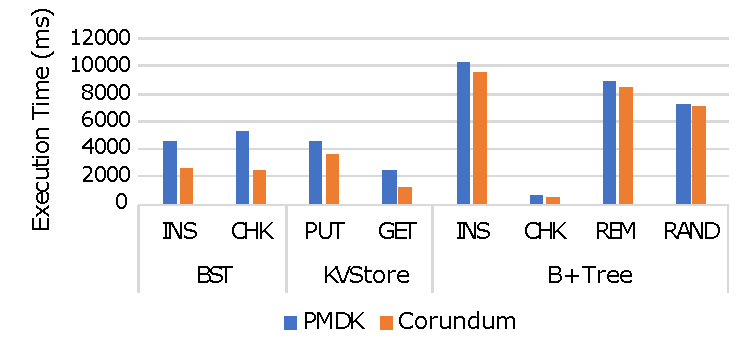
\includegraphics[width=3.3in]{Graphs/perf-ext.pdf}
  \end{center}
  \vspace*{-\baselineskip}
  \caption{\label{fig:perf} Performance comparison between \this{} and PMDK}
\end{figure}

\begin{table*}[!ht]
  \center
  \small
  \begin{tabular}{m{3.5in}m{3.5in}}
    \begin{lstlisting}[escapechar=\#]
use std::rc::*;
use std::cell::*;
struct Node { val: i32,
  nxt: Rc<RefCell<Option<Node>>>
}
fn insert(&self, val: i32) {
#\hllr{\linewidth}#
  let mut nxt = self.nxt.borrow_mut();
  if let Some(n) = &*nxt {
    if n.val > val {
      *nxt = Some(Node { val,
        nxt: self.nxt.clone()
      })
    } else { n.insert(val); }
  } else {
    *nxt = Some(Node { val,
      nxt: Rc::new(RefCell::new(None))
    })
  }
#\hllr{\linewidth}#
}\end{lstlisting}
    &
      \begin{lstlisting}[escapechar=\#]
use crndm::default::*;

struct Node { val: i32,
#\hll{\linewidth}#  nxt: #\hlw{15pt}#Prc<#\hlw{36pt}#PRefCell<Option<Node>>>
}
fn insert(&self, val: i32) {
#\hll{\linewidth}#  #\hlw{80pt}#transaction(|j| {
#\hll{\linewidth}#    let mut nxt = self.nxt.borrow_mut(#\hlw{5pt}#j);
    if let Some(n) = &*nxt {
      if n.val > val {
        *nxt = Some(Node { val,
#\hll{\linewidth}#          nxt: self.nxt.#\hlw{42pt}#pclone(j)
        })
      } else { n.insert(val); }
    } else {
      *nxt = Some(Node { val,
#\hll{\linewidth}#        nxt:#\hlw{15pt}#Prc::new(#\hlw{38pt}#PRefCell::new(None,#\hlw{5pt}#j),#\hlw{5pt}#j)
      })
    }
#\hll{\linewidth}#  #\hlw{52pt}#}).unwrap()
}\end{lstlisting}
  \end{tabular} 
  \vspace*{-\baselineskip}
  \caption{Comparing the implementation of insert operation in Rust and \This}
  \label{tbl:example}
\end{table*}
\vspace*{-\baselineskip}

\section{Key Results and Contributions}
\label{sec:key-contributions}

We have implemented \this{} and found its
performance to be as good or better than Intel's widely-used PMDK library.
\This{} enforces five invariants on PM programs:

\begin{enumerate}

\item PM pools only contain data that can be safely persistent.
\item Pointers within a pool are always valid.  Pointers between pools or from
  persistent memory to volatile memory are not possible.  Pointers from
  volatile memory into a pool are safe.  Closing a pool does not result in
  unsafe pointers.
\item  Transactions are atomic with respect to both persistent and volatile data.
  It is not possible to modify persistent data without logging
  it.
\item There are no data races or unsynchronized access to shared persistent data. 
\item Transactions provide isolation so that updates are not visible until the transaction commits. 
% \item Memory leaks and multiple frees are not possible. 
\end{enumerate}

\noindent
In almost every case, the compiler can statically detect violations of these
invariants.  \reftab{tab:libs} compares \this{}'s approach to preventing errors
with other PM libraries.  \This{} has much wider static coverage than any
existing system.

We compare \this{}'s performance to PMDK (Intel's optimized PM library) in
\reffig{fig:perf}.  The data show that \this{} is as fast or faster than PMDK
while still providing stronger safety guarantees.  

\begin{comment}
\section{Why ASPLOS?}
\label{sec:why-asplos}

\This{} applies recent developments in programming languages (i.e., Rust) to
persistent memory programming, an area of active architecture and systems
research.

\section{Citation for Most Influential Paper Award}
\label{sec:citation}

ASPLOS 2021's ``\papertitle'' is awarded the ASPLOS Most Influential Paper Award
for demonstrating the practicality of static verification of PM safety
properties.  The work laid the foundations for broader efforts in formal
verification of PM programs, and ultimately played a key role in making
wide-spread deployment of PM as a reliable and trustworthy storage technology feasible.



We also implemented
identical data structures in both libraries and compared the lines of code (LOC) required
add persistence (\reftab{tab:loc}).  \This{} required fewer lines of code in both relative and absolute terms.

\begin{table}%[!ht]
  \center
  \small
  \begin{tabular}{|r||c|c||c|c|}
      \hline
       & Rust & w/\This{} & C++ & w/PMDK \\ \hline\hline
      Linked List & 192&+19 (9.9\%) & 146&+45 (30.8\%)  \\ \hline
      Binary tree & 256&+12 (4.7\%) & 208&+41 (19.7\%) \\ \hline
      HashMap     & 165&+10 (6.1\%)  & 137&+42 (30.7\%) \\ \hline
  \end{tabular}
  \caption{Adding persistence to data structures with \this{} requires fewer changes (measured in lines of code) than PMDK.}
  \label{tab:loc}
\end{table}

\section{Why ASPLOS?}
\label{sec:why-asplos}

\This{} applies recent developments in programming languages (i.e., Rust) to
persistent memory programming, an area of active architecture and systems
research.

\section{Citation for Most Influential Paper Award}
\label{sec:citation}

ASPLOS 2021's ``\papertitle'' is awarded the ASPLOS Most Influential Paper Award
for demonstrating the practicality of static verification of PM safety
properties.  The work laid the foundations for broader efforts in formal
verification of PM programs, and ultimately played a key role in making
wide-spread deployment of PM as a reliable and trustworthy storage technology feasible.

ASPLOS emphasizes multidisciplinary research; explain how this
  paper emphasizes synergy of \emph{two or more ASPLOS areas}: architecture,
  programming languages, operating systems, and related areas (broadly
  interpreted).

\noindent
If you are unsure whether your paper falls within the scope of ASPLOS,
please check with the program chairs -- ASPLOS is a broad,
multidisciplinary conference and encourages new topics.

\section{Citation for Most Influential Paper Award}
\label{sec:citation}

Provide the citation for your paper if it won a Most Influential
Paper award. You can find example citations
on the \href{https://www.sigops.org/awards/hof/}{SIGOPS Hall of Fame}
and \href{https://www.sigplan.org/Awards/PLDI/}{PLDI most influential
  paper list}.  Limit the citation to 1-3 sentences
\emph{Recall that your citation here must be anonymous}; do not include names or affiliations.

%  \url{https://rb.gy/hd1hms}).

\section{Revisions}
\label{sec:revisions}

 \emph{Optional:} Describe how this paper has been revised, if it was previously submitted to another conference.
\end{comment}

 
% \pagebreak
\bibliographystyle{abbrv}
\bibliography{paper,libpaper/common}


\end{document}
